\documentclass[11pt,a4paper]{report} 

\usepackage[utf8]{inputenc}
\usepackage{fancyhdr}
\usepackage{graphicx}
\usepackage{lipsum}
\usepackage{tikzpagenodes}
\usepackage{lastpage}
\usepackage{fancyheadings}
\usepackage{tabularx}
\usepackage{xcolor}
\usepackage{amsmath}
\usepackage{tikzpagenodes}
\usepackage[ddmmyyyy]{datetime}
\usepackage[toc,acronym,nopostdot,nonumberlist]{glossaries}
\usepackage[margin=3cm]{geometry}
\usepackage[hidelinks]{hyperref}

\usepackage{amsfonts}
\usepackage{csquotes}
\usepackage{comment}
\usepackage{imakeidx}
\usepackage{multirow}
\usepackage{titling}
\usepackage[T1]{fontenc}
\usepackage[french]{babel} 
\usepackage{listings}
\usepackage[autolanguage]{numprint}
\usepackage{hyperref}
\usepackage{caption}

\usepackage{tikz}
\usepackage{xparse}
\usepackage{float}

\usepackage{verbatim}

\usepackage{bigints}
\usepackage{bm}
\usepackage[nottoc, notlof, notlot]{tocbibind}

\usepackage{tcolorbox}
\usepackage{siunitx}


\def\code#1{\texttt{#1}}


\newcommand\blfootnote[1]{%
  \begingroup
  \renewcommand\thefootnote{}\footnote{#1}%
  \addtocounter{footnote}{-1}%
  \endgroup
}

%%%%%%%%%%%%%%%%%%%




\lstset{%
  language=Ada,
  basicstyle   = \ttfamily,
  keywordstyle =    \color{violet},
  keywordstyle = [2]\color{violet},
  commentstyle =    \color{teal},
  stringstyle  =    \color{olive},
  numbers      = left,
  frame        = single,
  framesep     = 2pt,
  aboveskip    = 1ex
}

\hypersetup{
    colorlinks=true,
    linkcolor=blue,
    }

\makeatletter
\@addtoreset{chapter}{part}
\makeatother  



\begin{document} 
\begin{titlepage}
\begin{tikzpicture}[remember picture,overlay,shift={(current page.center)}]
\node[anchor=center,xshift=0cm,yshift=13cm]{
\includegraphics[scale=0.3]{ENSEEIHT_logo.png}};
\end{tikzpicture}
\centering
\vspace{2.5cm}
\huge
\\ Rapport \\
\vspace{1cm}
\begin{center}
\textbf{Introduction à la synchronisation} \\ Impact d’une erreur de phase porteuse et méthode de récupération
\end{center}

\vspace{1cm}
\large \textit{réalisé par}\\
\vspace{0.2cm}
\Large Samy Afker \& Maxime Moshfeghi\\


\begin{figure}[ht]
    \centering
    
\includegraphics[width=0.6\textwidth]{modem.png}
    \label{fig:Routeur}  
\end{figure}

\vspace{2cm}
ENSEEIHT - 1SN - Télécommunications -
\vspace{0.5cm}
2022 - 2023

\end{titlepage}


\pagestyle{fancy}
\renewcommand\headrulewidth{1pt}
\fancyhead[L]{\nouppercase{\leftmark}}
\fancyhead[R]{Rapport Projet}
\renewcommand\footrulewidth{1pt}
\fancyfoot[C]{S. Afker - M. Moshfeghi\\
\vspace{0.1cm}
\textbf{\thepage}}
\fancyfoot[L]{Télécommunications}
\renewcommand\thesection{\arabic{section}}

\fancyfoot[R]{2022 - 2023}

\tableofcontents

%%%%%%%%%%%%%%%%%%%%%%%%%%%%%%%%%%%%%%%%%%%%%%%%%%%%%%%%%%%%%%%%%%%%

%                                                                  %

%%%%%%%%%%%%%%%%%%%%%%%%%%%%%%%%%%%%%%%%%%%%%%%%%%%%%%%%%%%%%%%%%%%%
\renewcommand\thesection{\arabic{section}}

\part{Introduction}

$~$

\vspace{6.5cm}


L'idée de cette partie est de visualiser l'impact d'une erreur de phase porteuse sur un signal reçu, et d'élaborer une approche afin de résoudre les problèmes que cela peut engendrer à sa réception. La chaîne équivalente implantée sera donc la suivante :
\begin{figure}[H]
    \centering
    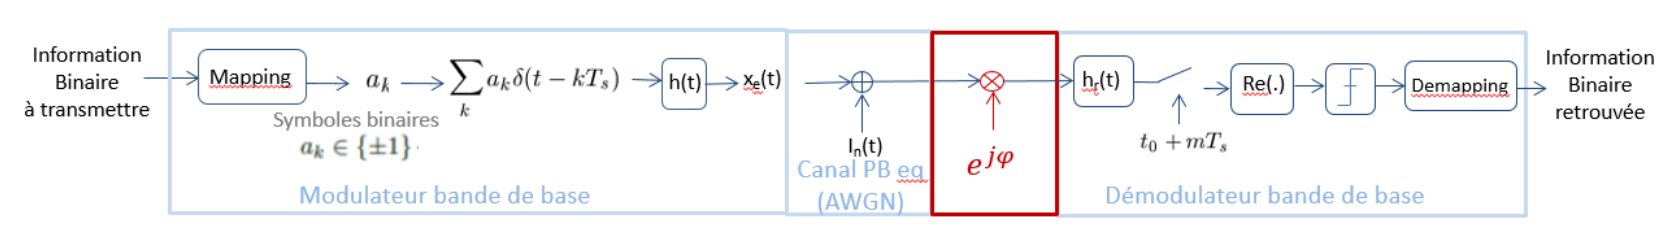
\includegraphics[width=15 cm]{Screenshots/schema.png}
    \caption{Chaîne de transmission passe-bas équivalente avec erreur de phase porteuse $\varphi$}
    \label{fig:un_label} 
\end{figure}

\vspace{0.3cm}

Dans un premier temps, nous verrons comment un déphasage peut agir sur la taux d'erreur binaire à la réception. On s'intéressera ensuite à une première version de résolution de ce déphasage grâce à un estimateur : l'\textbf{estimateur de Viterbi et Viterbi}. Enfin, après avoir décrit les limites de cet estimateur, nous verrons une méthode supplémentaire pour s'affranchir de toute erreur sur la phase porteuse (dans le cadre du TP) : le \textbf{codage par transition}.



\part{Impact d'une erreur de phase porteuse}

\chapter{Étude théorique}

% Question 2.1.1

\section{Respect du critère de Nyquist}

La réponse impulsionnelle globale du filtre $g(t) = h(t) \ast h_r(t)$ est la suivante :

\begin{center}
    $\Pi_{T_s}\displaystyle\left(t - \cfrac{T_s}{2}\right) \ast \Pi_{T_s}\displaystyle\left(t - \cfrac{T_s}{2}\right) = \Lambda_{T_s}\displaystyle\left(t - T_s\right)$
\end{center}

\begin{tcolorbox}[colback=blue!5!white,
                  colframe=blue!75!black,
                  title=Notations
                 ]
On s'accorde à noter $\Pi_{T_s}$ la fonction porte de largeur $T_s$ de hauteur 1 centrée en 0 et $\Lambda_{T_s}$ la fonction triangle de largeur $2T_s$ (de hauteur maximale $T_s$) centrée en 0.
\end{tcolorbox}
Afin de respecter le critère de Nyquist, il faut donc échantillonner à $T_s + mT_s$.

\newpage

% Question 2.1.2
\vspace{0.5cm}

\section{Expression du signal en sortie d'échantillonneur}

Avec une erreur sur la phase porteuse de $\varphi$, on peut donner l'expression du signal en sortie de l'échantilloneur qui en résulte :

\begin{tcolorbox}[colback=black!5!white,
                  colframe=black!70!white,
                  title=Cheminement du signal à travers la chaîne,
                  fonttitle=\bfseries,
                    subtitle style={boxrule=0.4pt,
                    colback=black!50!white!25!white,
                    colupper=black!90!white}
                 ]
    \tcbsubtitle{À l'entrée de la chaîne} 
    Suite de bits $\beta_k \in \{0,1\}.$ 
    \tcbsubtitle{Après mapping} 
    Suite de symboles $a_k \in \{-1,1\}$.
    \tcbsubtitle{Après suréchantillonnage}
    $\sum\limits_{k} a_k \delta\displaystyle\left(t - kT_s\right)$
    \tcbsubtitle{Après mise en forme}
    $\sum\limits_{k} a_k h\displaystyle\left(t - kT_s\right)$
    \tcbsubtitle{Ajout d'un bruit gaussien}
    $\sum\limits_{k} a_k h\displaystyle\left(t - kT_s\right) + I_n(t)$
    \tcbsubtitle{Ajout d'une erreur de phase porteuse}
    $\displaystyle\left(\sum\limits_{k} a_k h\displaystyle\left(t - kT_s\right) + I_n\displaystyle\left(t\right)\right)e^{j\varphi} = e^{j\varphi}\sum\limits_{k} a_k h\displaystyle\left(t - kT_s\right) + I_n\displaystyle\left(t\right)e^{j\varphi}$
    \tcbsubtitle{Réception du signal}
    $e^{j\varphi}\sum\limits_{k} a_k h \ast h_r \displaystyle\left(t - kT_s\right) + I_w = e^{j\varphi}\sum\limits_{k} a_k \Lambda_{T_s} \displaystyle\left(t - kT_s\right) + I_w$
    \tcbsubtitle{Échantillonnage à $t_0 + mT_s$ avec $t_0 = T_s$}
    $e^{j\varphi}\sum\limits_{k} a_k \underbrace{\Lambda_{T_s} \displaystyle\left(t - kT_s\right) \delta\displaystyle\left(t - kT_s\right)}_{= \Lambda_{T_s} \displaystyle\left(kT_s\right) \delta\displaystyle\left(t - kT_s\right)} + I_w = e^{j\varphi}\sum\limits_{k} a_k T_s \delta\displaystyle\left(t - kT_s\right) + I_w$
\end{tcolorbox}

On obtient donc, après échantillonage :
\begin{center}
$~$
$z(t) = e^{j\varphi}\sum\limits_{k} a_k T_s \delta\displaystyle\left(t - kT_s\right) + I_w$
\end{center}


% Question 2.1.3
\vspace{0.5cm}

\section{Calcul du TEB théorique du signal avec erreur de phase}

On va maintenant calculer le TEB théorique d'une telle chaîne de transmission.
\newline
On a l'expression suivante :
\begin{align*}
    TEB & = Q\displaystyle\left(\cfrac{D_{min}}{2\sigma_{I_w}}\right)
\end{align*}

$D_{min}$ étant la distance minimale entre deux symboles différents après décision, dû à l'erreur sur la phase porteuse $\varphi$, cette quantité est la suivante :
\begin{align*}
    D_{min} & = \mathfrak{Re}\displaystyle\left( e^{j\varphi} a_1 T_s - e^{j\varphi} a_0 T_s \right) = \mathfrak{Re}\displaystyle\left( e^{j\varphi}T_s + e^{j\varphi}T_s \right) = \mathfrak{Re}\displaystyle\left( 2e^{j\varphi}T_s \right) = 2T_s\cos\varphi 
\end{align*}

On en déduit :

\begin{align*}
    TEB & = Q\displaystyle\left(\cfrac{T_s\cos\varphi}{\sigma_{I_w}}\right)
\end{align*}

% Question 2.1.4
\vspace{0.5cm}

\section{Calcul de $\sigma_{I_w}^{~2}$}

On peut maintenant calculer la valeur de $\sigma_{I_w}$. Dans un premier temps, on a d'après Wiener-Lee :

\begin{align*}
    I_w(f) & = I_n \displaystyle\left\lvert H_r(f) \right\rvert^2 = \cfrac{N_0}{2}\displaystyle\left\lvert H_r(f) \right\rvert^2
\end{align*}

D'où :

\begin{align*}
    \hspace{3cm} \sigma_{I_w}^{~2} & = \displaystyle \int_{\mathbb{R}}I_w(f)df & \\
    & = \cfrac{N_0}{2} \displaystyle \int_{\mathbb{R}} \displaystyle\left\lvert H_r(f) \right\rvert^2 df & \\
    & = \cfrac{N_0}{2} \underbrace{\displaystyle\int_{\mathbb{R}} \displaystyle\left\lvert h_r(t) \right\rvert^2 dt}_{T_s} & \text{(Parseval)}
\end{align*}

Donc :

\begin{align*}
    \sigma_{I_w}^{~2} = \cfrac{N_0T_s}{2}
\end{align*}

% Question 2.1.5
\vspace{0.5cm}

\section{Calcul de $E_s$}

On peut maintenant calculer l'énergie symbole $E_s$. On a :

\begin{align*}
    E_s & = P_xT_s
\end{align*}

Avec :

\begin{align*}
    P_x & = \displaystyle\int_{\mathbb{R}} S_x(f) df
\end{align*}

On a alors :

\begin{align*}
    \hspace{5.5cm} m_a & = \cfrac{1}{2}(1) + \cfrac{1}{2}(-1) = 0 & \hspace{1cm} \text{(mapping à moyenne nulle)}
\end{align*}

\newpage

\begin{align*}
    \sigma_a^2 & = \cfrac{1}{2}(1)^2 + \cfrac{1}{2}(-1)^2 - 0 = 1
\end{align*}

L'expression de la DSP se simplifie donc de la manière suivante :
\blfootnote{1. Avec $\mathbb{E}\displaystyle\left[a_m^*a_{m-k} \right] \, = \, 0 ~ \forall k \in \mathbb{N^*}$ et $m_a \, = \, 0$, on a $\forall k \in \mathbb{N^*}, \, R_a(k) \, = \, 0$ }

\begin{align*}
S_{x}(f) = & \, \cfrac{\sigma_a^2}{T_s} \displaystyle\left\lvert H(f)\right\rvert ^2 + \underbrace{2 \cfrac{\sigma_a^2}{T_s} \displaystyle\left\lvert H(f)\right\rvert ^2 \sum_{k=1}^{\infty}\mathfrak{Re}\displaystyle\left[R_a(k)e^{j2\pi fkT_s}\right]}_{= \, 0 \text{ car } \forall k \in \mathbb{N^*}, ~ R_a(k) \, = \, 0 \footnotemark} + \underbrace{\cfrac{|m_a|^2}{T_s^2}\sum_k \displaystyle\left\vert H\displaystyle\left( \cfrac{k}{T_s}\right)\right\vert ^2\delta\displaystyle\left(f - \cfrac{k}{T_s}\right)}_{= \, 0 \text{ car } m_a \, = \, 0}
\end{align*}

Donc : 

\begin{center}
    $S_{x}(f) = \, \cfrac{1}{T_s} \displaystyle\left\lvert H(f)\right\rvert ^2$
\end{center}

Ainsi : 

\begin{align*}
    P_x & = \displaystyle\int_{\mathbb{R}} S_x(f) df = \cfrac{1}{T_s} \underbrace{\displaystyle\int_{\mathbb{R}} \displaystyle\left\lvert H(f)\right\rvert ^2 df}_{T_s} = 1
\end{align*}

On a donc :

\begin{center}
    $E_s = T_s$
\end{center}


% Question 2.1.6
\vspace{0.5cm}

\section{Expression finale du $TEB$}

Comme $R_b = R_s$ (mapping binaire), on en déduit :
\begin{center}
    $E_b = E_s$
\end{center}

Ainsi, on déduit la formule du taux d'erreur binaire suivante :

\begin{align*}
    TEB & = Q\displaystyle\left( T_s\cos\varphi\sqrt{\cfrac{2}{N_0T_s}} \right) = Q\displaystyle\left( \cos\varphi\sqrt{\cfrac{2T_s}{N_0}} \right)
\end{align*}

Donc :

\begin{align*}
    TEB & = Q\displaystyle\left( \cos\varphi\sqrt{\cfrac{2E_b}{N_0}} \right)
\end{align*}


\chapter{Implantation sous Matlab}

% Question 2.2.1

% Question 2.2.2
% TODO épaisseur points

\section{Implantation de la chaîne sans erreur de phase et sans bruit}

\begin{figure}[H]
    \centering
    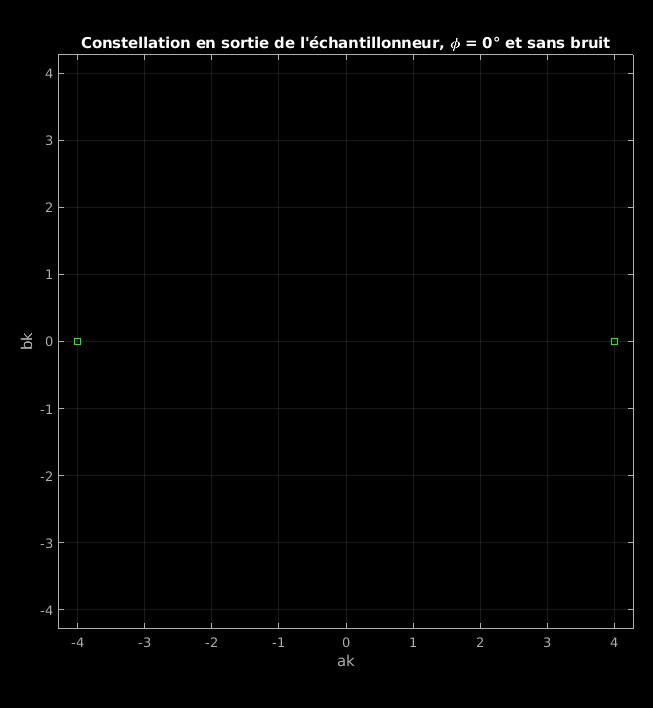
\includegraphics[width=7 cm]{Screenshots/2_2_1.jpg}
    \caption{Constellation après échantillonage pour une erreur sur la phase nulle}
    \label{fig:un_label} 
\end{figure}


%\begin{figure}[H]
%    \centering
%    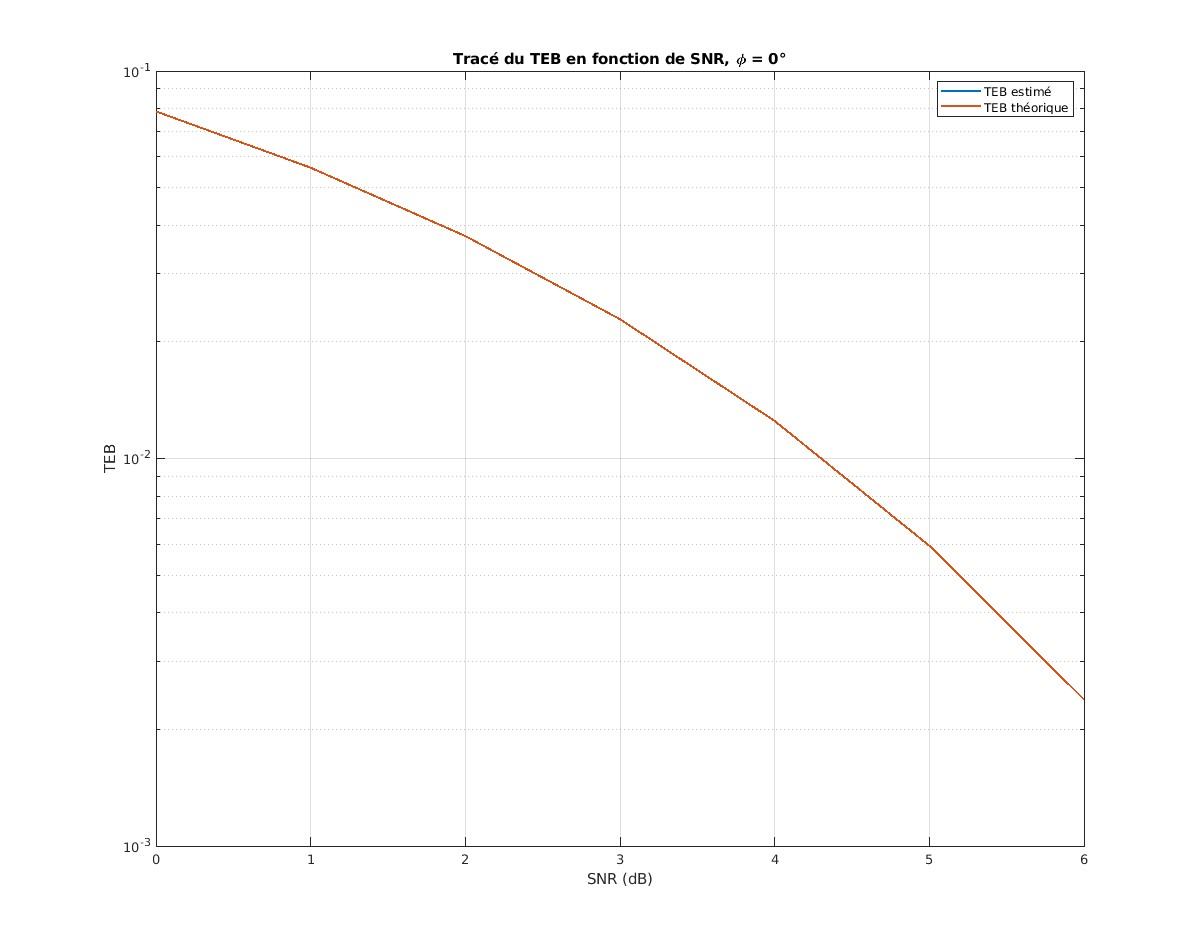
\includegraphics[height=8 cm]{Screenshots/2_2_2.jpg}
%    \caption{TEB obtenu pour la chaîne de transmission sans bruit et sans déphasage}
%    \label{fig:un_label} 
%\end{figure}

\begin{table}[H]
        \centering
        \fontsize{12}{20}\selectfont
        \caption{TEB obtenu sans déphasage et sans bruit}
        \label{tableau_power}
        \makebox[\linewidth]{
        \begin{tabular}{|c|c|}
            \hline
             $\varphi$ & 0 \\
            \hline
             $TEB$ & 0 \\
            \hline
        \end{tabular}
        }
\end{table}

On trouve bien un TEB nul.

% Question 2.2.3

\section{Implantation de la chaîne avec erreur de phase et sans bruit}

\begin{figure}[H]
    \centering
    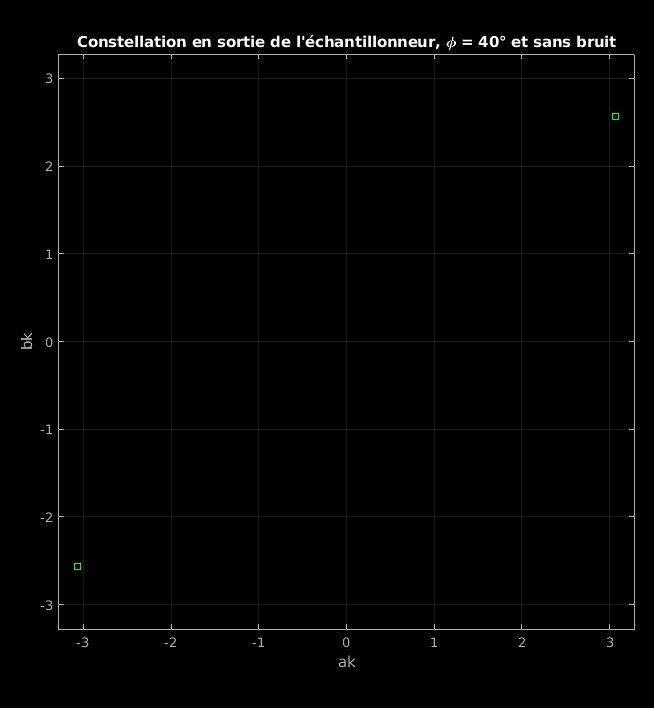
\includegraphics[height=5.3 cm]{Screenshots/2_3_1.jpg}
    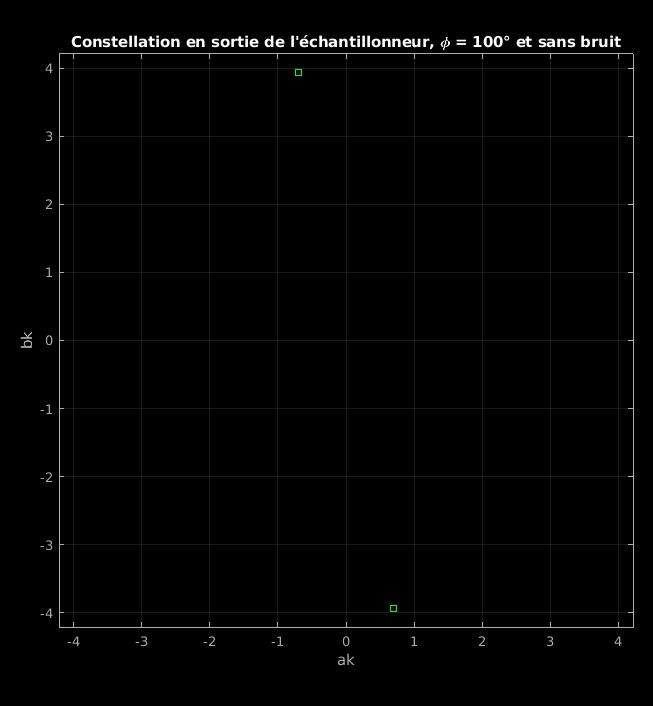
\includegraphics[height=5.3 cm]{Screenshots/2_3_2.jpg}
    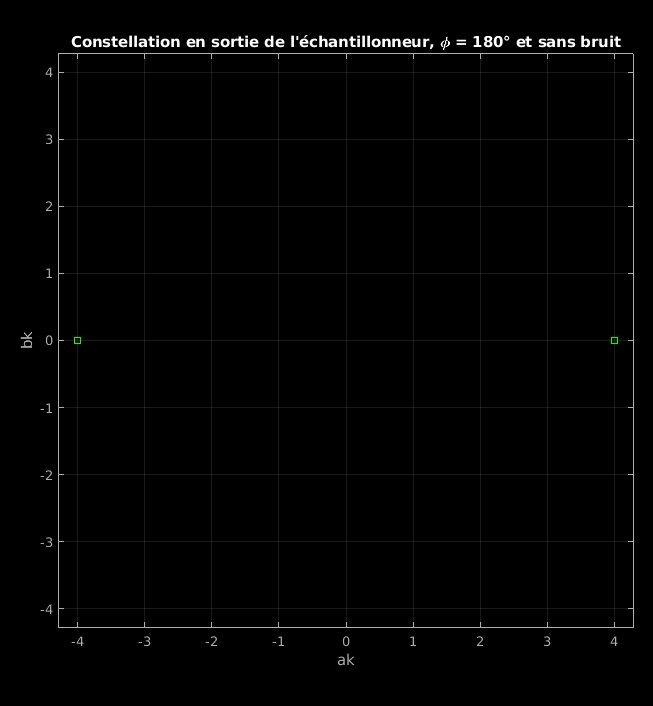
\includegraphics[height=5.3 cm]{Screenshots/2_3_3.jpg}
    \caption{Constellations après échantillonage pour une erreur sur la phase de 40°, 100° et 180°}
    \label{fig:un_label} 
\end{figure}

%\begin{figure}[H]
%    \centering
%    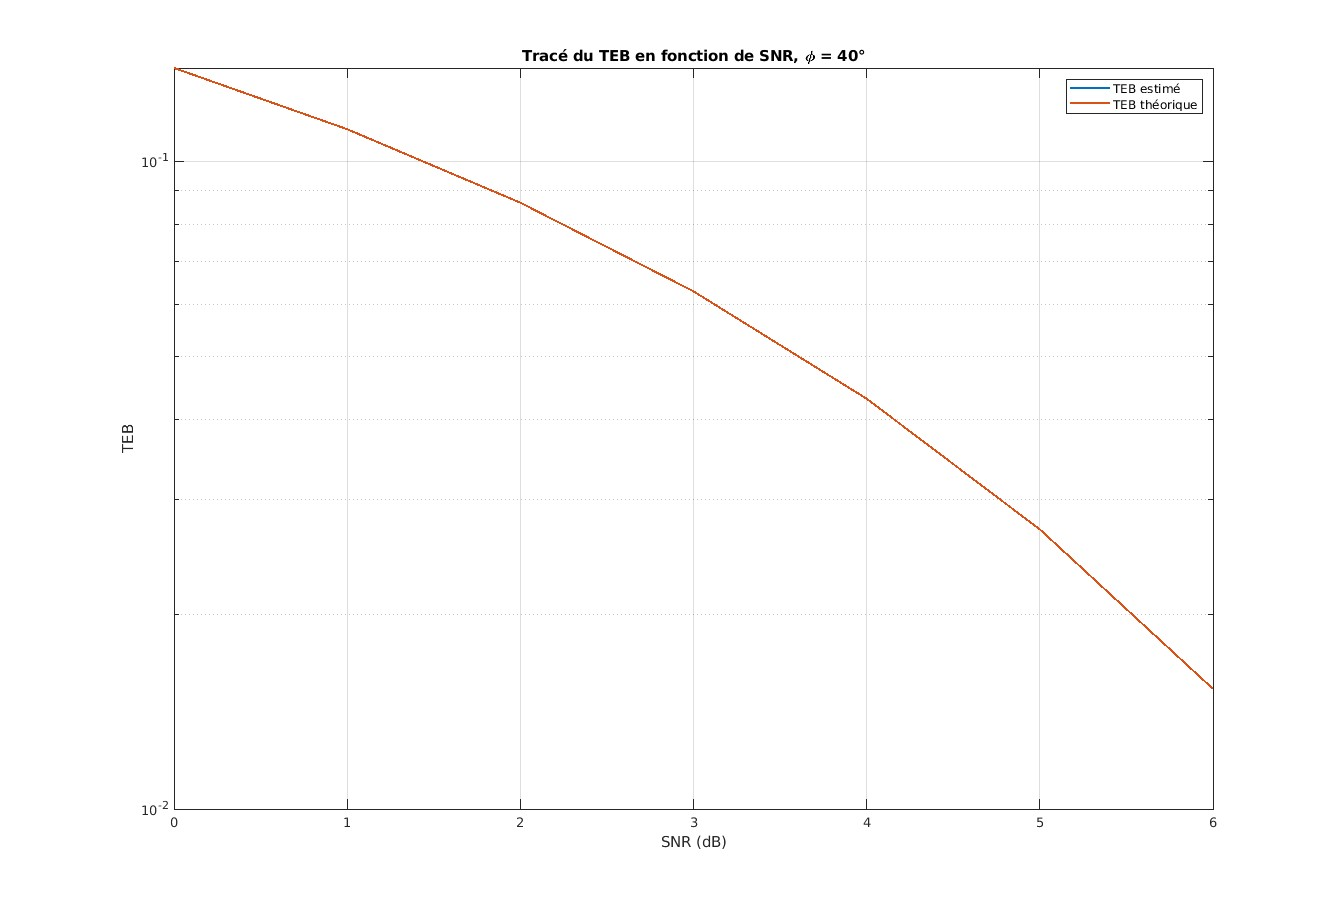
\includegraphics[height=7.5 cm]{Screenshots/2_3_4.jpg}
%    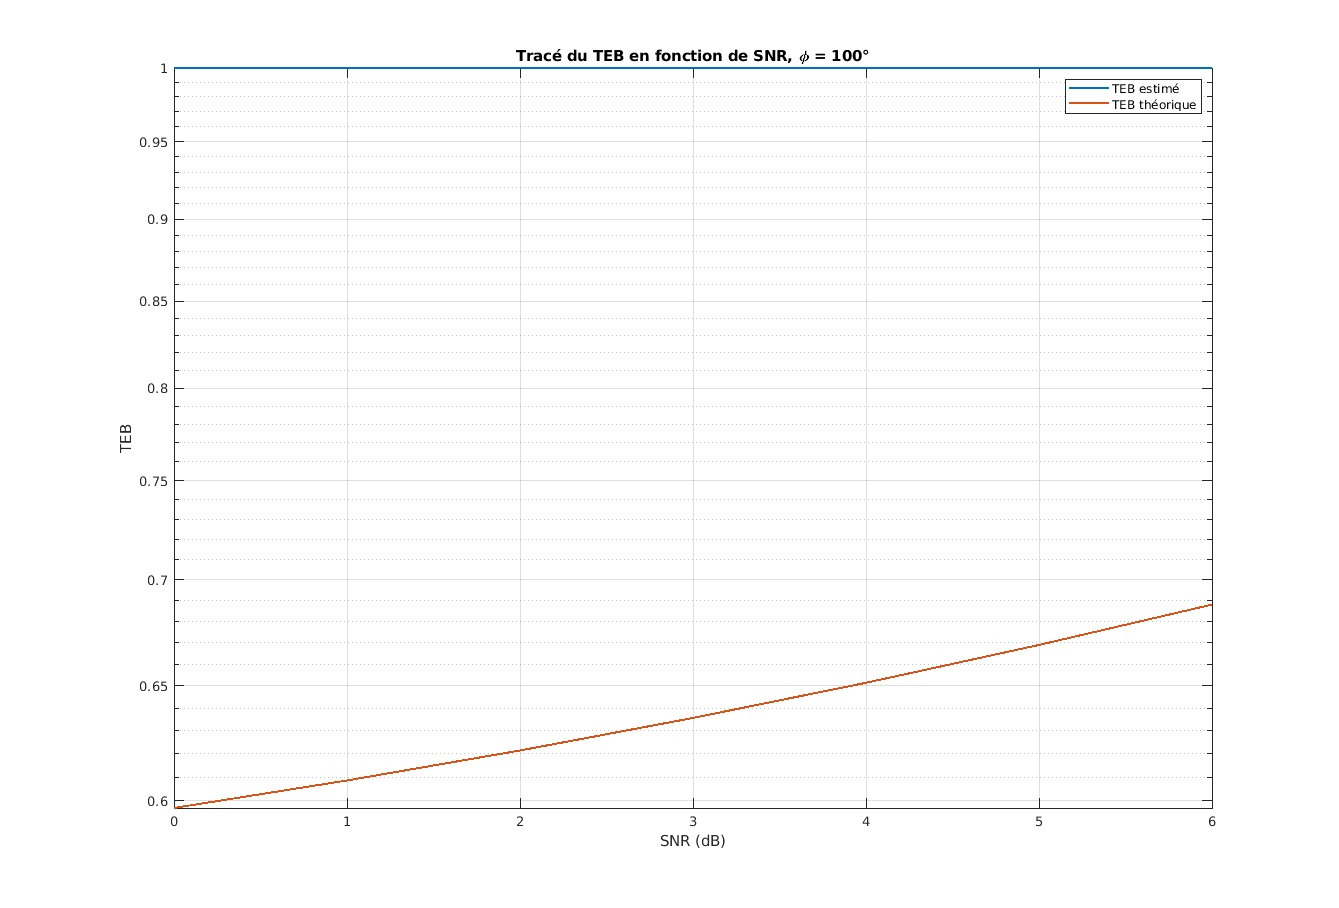
\includegraphics[height=7.5 cm]{Screenshots/2_3_5.jpg}
%    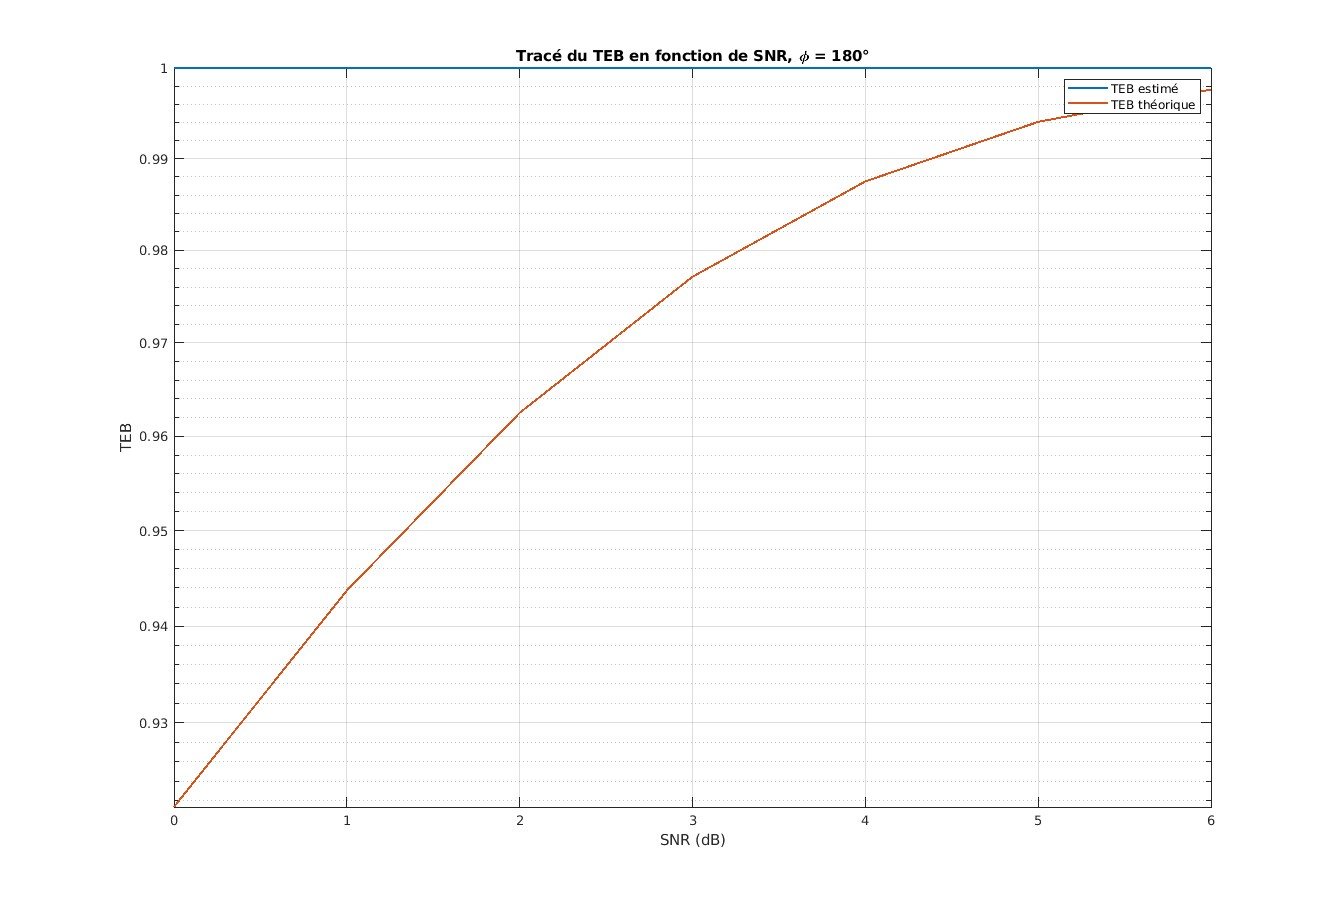
\includegraphics[height=7.5 cm]{Screenshots/2_3_6.jpg}
%    \caption{TEB obtenus pour une erreur sur la phase de 40°, 100° et 180°}
%    \label{fig:un_label} 
%\end{figure}

\begin{table}[H]
        \centering
        \fontsize{12}{20}\selectfont
        \caption{TEB obtenu sans déphasage et sans bruit}
        \label{tableau_power}
        \makebox[\linewidth]{
        \begin{tabular}{|c|c|c|c|}
            \hline
             $\varphi$ & 40 & 100 & 180 \\
            \hline
             $TEB$ & 0 & 1 & 1 \\
            \hline
        \end{tabular}
        }
\end{table}


Pour le cas $\varphi = 40$°, on observe que les TEB simulé est nul.
\newline
En revanche, pour les TEB simulés et théoriques tracés pour des erreurs de phase de $\varphi = 100$° et $\varphi = 180$°, les TEB sont désormais égaux à 1. Cela s'explique par le fait que lors de la démodulation, les signaux initialement mappés sur le symbole -1 vont être attribué lors de la décision à 1, et vice-versa. De manière générale, sans correction sur la phase et sans ajout de bruit, on aura :

\begin{align*}
    k \in \mathbb{Z}, \forall \varphi \in \displaystyle\left] \cfrac{k\pi}{2} , ~ \cfrac{3k\pi}{2} \right[, ~ TEB = 1
\end{align*}


% Question 2.2.4

\newpage

\section{Implantation de la chaîne avec erreur de phase et avec bruit}

On implante maintenant la chaîne de transmission complète avec erreur de phase et ajout de bruit.

% Question 2.2.4.a

\begin{figure}[H]
    \centering
    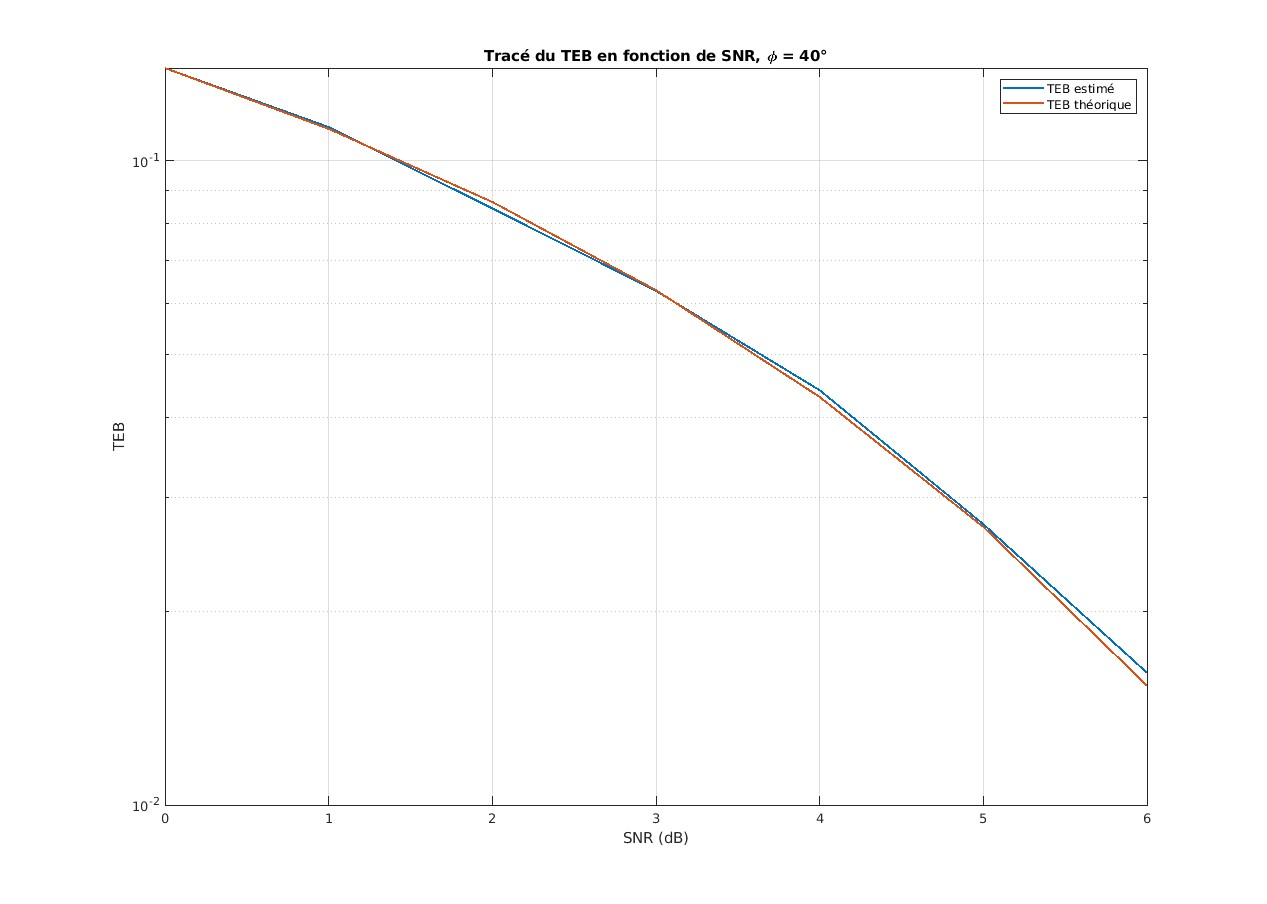
\includegraphics[height=7cm]{Screenshots/2_4_a.jpg}
    \caption{Comparaison du TEB théorique et simulé pour une erreur de phase $\varphi = 40$°}
    \label{fig:un_label} 
\end{figure}

On constate que la chaîne est bien fonctionnelle. En effet, les tracés des TEB théoriques et simulés pour $\varphi = 40$° sont supersposés.


% Question 2.2.4.b

\vspace{0.3cm}

On peut maitenant comparer les TEB obtenus avec et sans erreur de phase.


\begin{figure}[H]
    \centering
    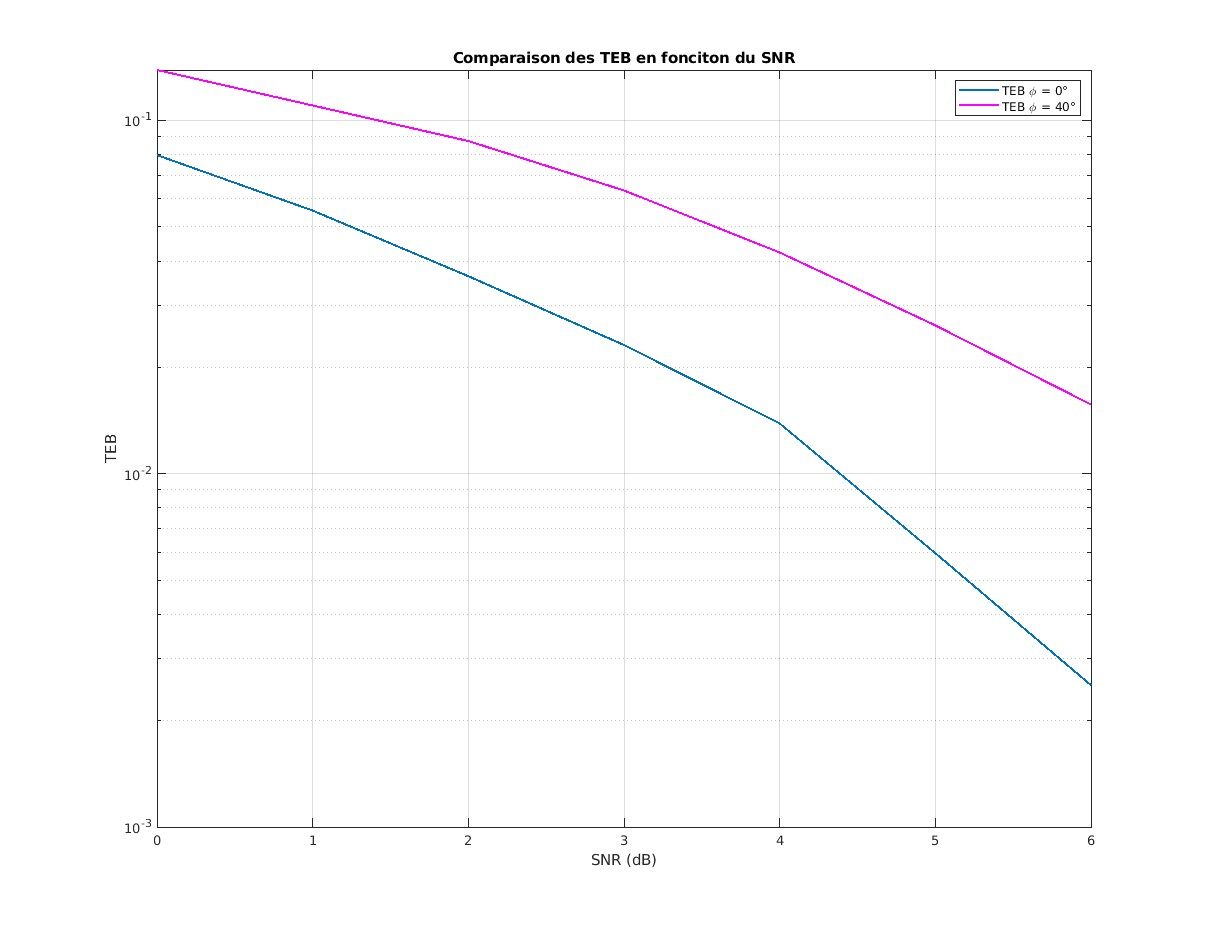
\includegraphics[height=7.5cm]{Screenshots/2_4_b.jpg}
    \caption{Comparaison des TEB simulés pour une erreur sur la phase de 0° et 40°}
    \label{fig:un_label} 
\end{figure}

On remarque que quelle que soit la valeur de SNR, le TEB est plus grand pour le signal déphasé de 40°.


% Question 2.2.4.c
\newpage

\vspace{0.3cm}

On peut aussi comparer les TEB obtenus pour deux erreurs de phases différentes.

\begin{figure}[H]
    \centering
    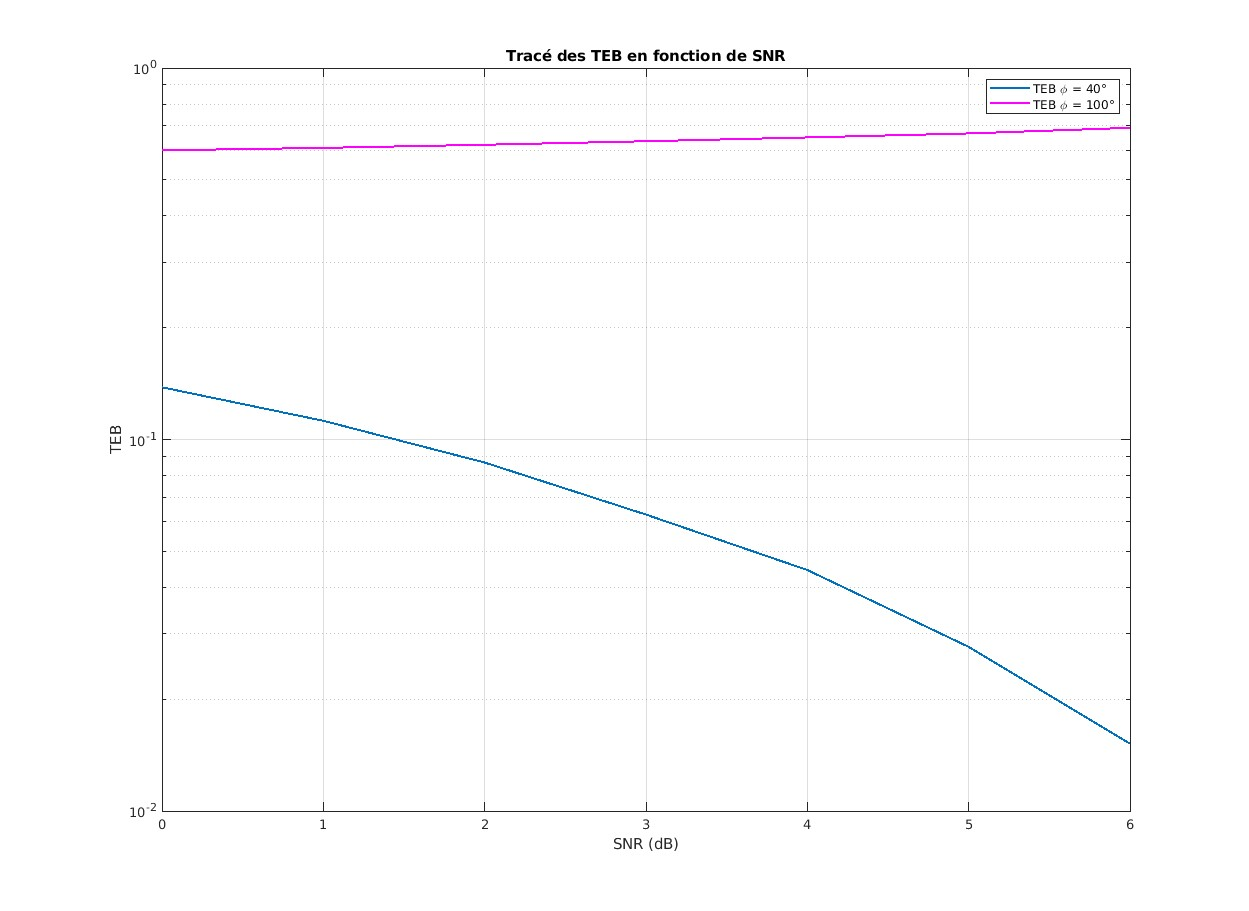
\includegraphics[height=7cm]{Screenshots/2_4_c.jpg}
    \caption{Comparaison des TEB simulés pour une erreur sur la phase de 40° et 100°}
    \label{fig:un_label} 
\end{figure}


% Question 2.2.4.d

Cette fois-ci, la courbe du TEB pour $\varphi = 100$° est croissante avec SNR. Cela est dû fait que les décisions ne sont plus faites correctement. En effet, cela est du au fait que lors de la projection sur l'axe des réels des données post-échantillonnage, les points normalement mappés sur 1 se trouvent dans la partie des réels négatifs, et ceux mappés sur -1 se trouvent dans la partie des réels positifs. En découle une erreur de décision, ce qui a donc un impact direct sur le TEB.



\part{Estimation et correction de l’erreur de phase porteuse}

%\chapter{Étude théorique}


\chapter{Implantation sous Matlab}

% Question 3.2.1

\begin{table}[H]
        \centering
        \fontsize{12}{20}\selectfont
        \caption{Comparaison de la phase appliquée et celle estimée pour la démodulation (en °)}
        \label{tableau_power}
        \makebox[\linewidth]{
        \begin{tabular}{|c|c|c|c|c|}
            \hline
             $\varphi$ & 0 & 40 & 100 & 180 \\
            \hline
             $\hat{\varphi}$ & -0.1396 & 40.0452 & -80.1172 & -0.0495 \\
            \hline
        \end{tabular}
        }
\end{table}

On remarque que pour $\phi = 0°$ et $\phi = 40°$ la phase estimée est bien estimée. Par contre, pour $\phi = 100°$ et $\phi = 180°$ on obtient $\phi - \pi$ (explication plus approfondie en fin de chapitre).


% Question 3.2.2

\vspace{0.3cm}

On va maintenant comparer le courbes avec et sans correction de phase.

\begin{figure}[H]
    \centering
    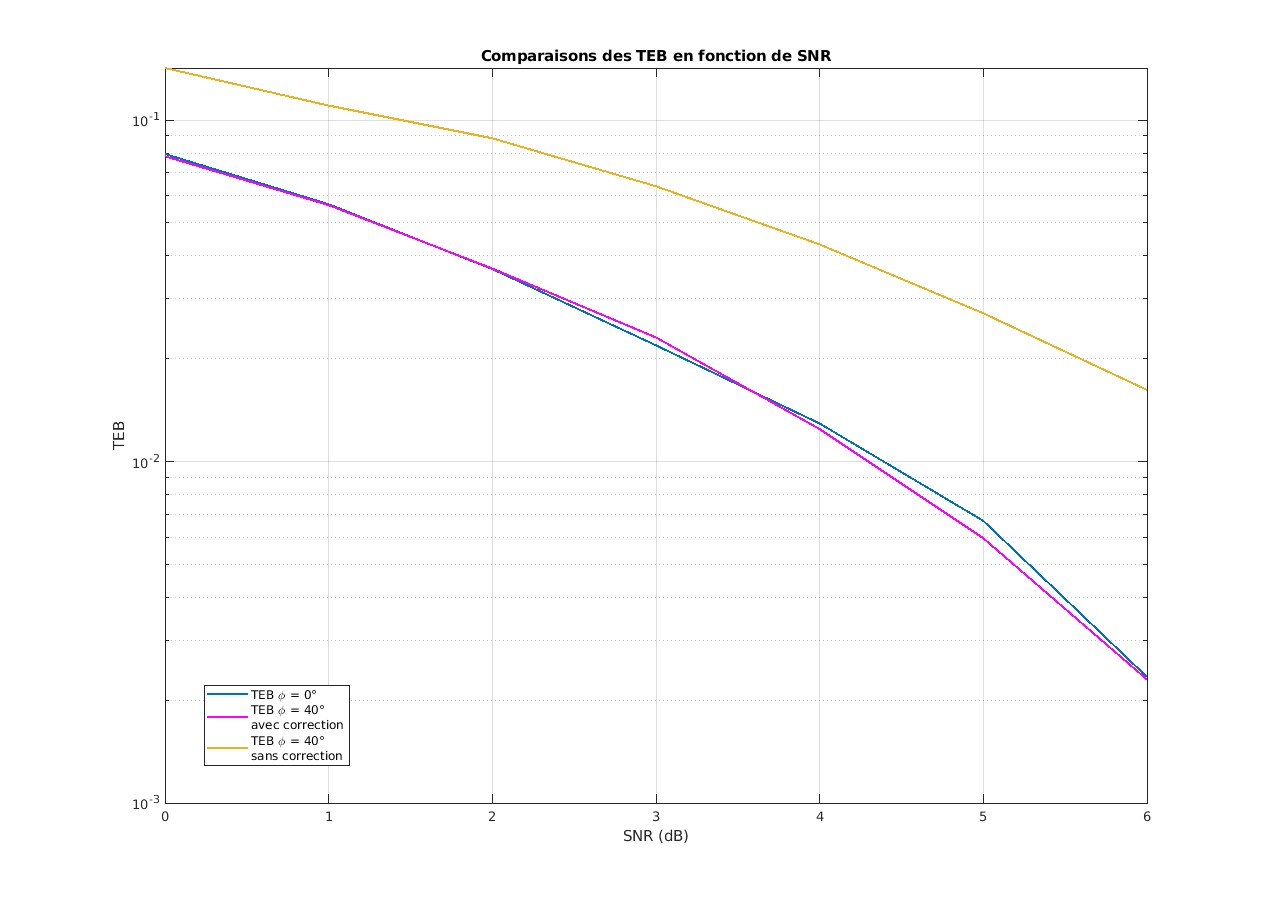
\includegraphics[height=10cm]{Screenshots/3_2_1.jpg}
    \caption{Comparaison des TEB simulés pour $\varphi = 40$° avec et sans correction d'erreur sur la phase avec le TEB simulé sans erreur de phase}
    \label{fig:un_label} 
\end{figure}

On remarque que les courbes de TEB sans déphasage et avec déphasage et correction de phase sont confondues. L'impact de l'erreur de phase (visible sur la courbe orange) a donc été corrigé dans ce cas (courbe rose).

\begin{figure}[H]
    \centering
    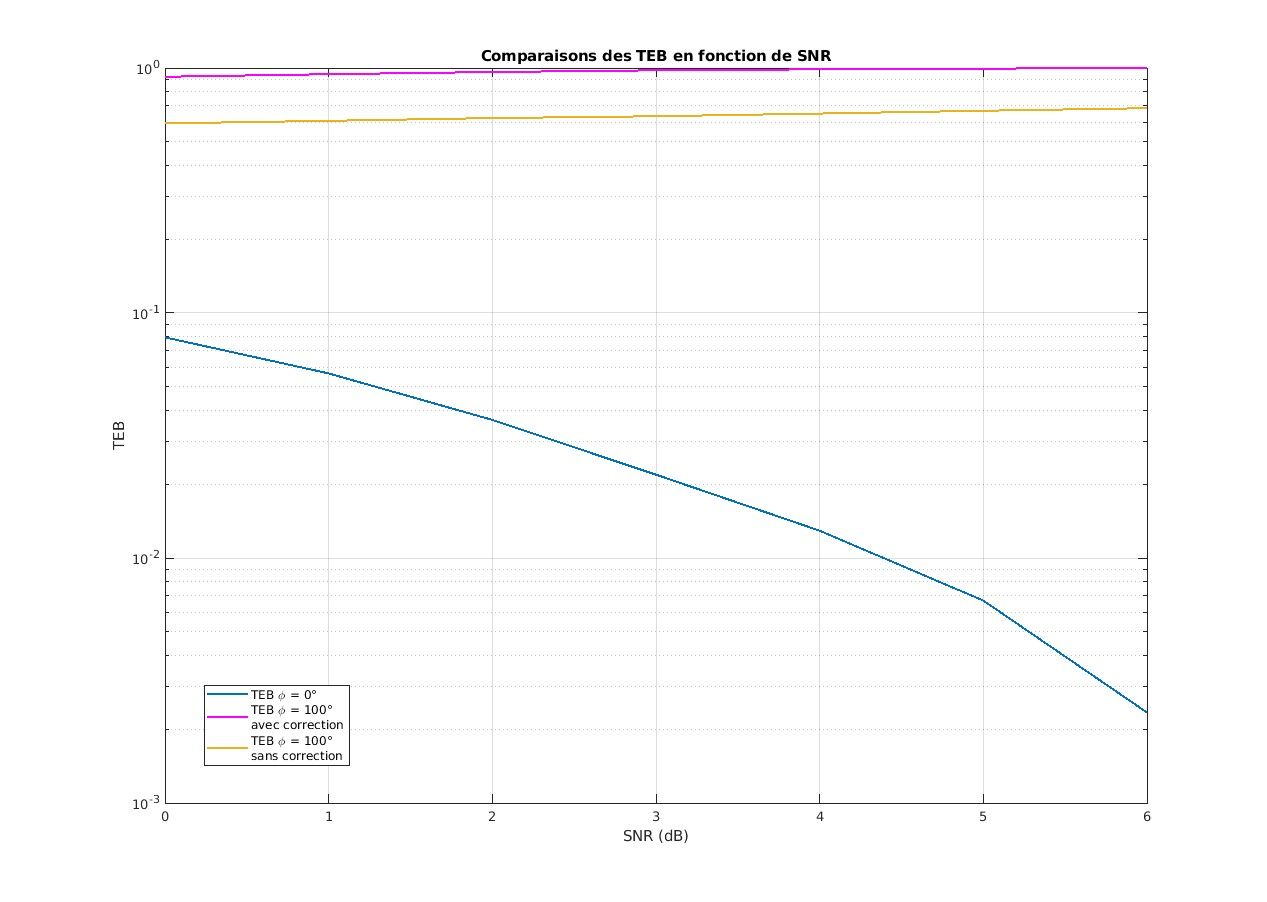
\includegraphics[height=10cm]{Screenshots/3_2_2.jpg}
    \caption{Comparaison des TEB simulés pour $\varphi = 100$° avec et sans correction d'erreur sur la phase avec le TEB simulé sans erreur de phase}
    \label{fig:un_label} 
\end{figure}

En revanche, pour une erreur sur la phase de $\varphi = 100$°, on remarque que cela ne fonctionne pas. En fait, on remarque surtout que la chaîne avec l'erreur de $\varphi = 100$° et correction donne un TEB proche de 1 (et croissant avec SNR). En fait, l'estimateur de Viterbi et Viterbi est préci à $\pi$ près. Ici, au lieu de trouver 100°, l'estimateur trouve -80°. Dans la correction de phase, au lieu de supprimer la phase de 100°, une phase de 80° va donc être ajouté, ce qui amène une phase totale de 180° au signal. Ainsi, la grande majorité des décisions se feront mal, ce qui amènera à une inversion bit à bit du signal.



\part{Utilisation d’un codage par transition}

\chapter{Étude théorique}

% Question 4.1.1
\section{Affranchissment de l'ambiguïté de $\pi$}

Après le décodage, on obtient des symboles décodés $\hat{a}_k$. Or, on a :

\begin{center}
    $\hat{a}_k = c_k \cdot c_{k-1} = (a_k \cdot c_{k-1}) \cdot c_{k-1} = a_k \cdot c_{k-1}^2 = a_k$.
\end{center}

Ainsi, le codage permet de retrouver les symboles $a_k$ initialement émis sans ambiguïté. 

% Question 4.1.2
\section{TEB des symboles codés}

Après le codage, on obtient des symboles $c_k$ qui s'expriment sous la forme :

\begin{center}
    $\hat{a}_k = c_k \cdot c_{k-1}$
\end{center}

Ainsi, un symbole $\hat{a}_k$ peut être erroné à cause d'une erreur sur $c_k$ ou à cause d'une erreur sur  $c_{k-1}$. On a donc deux fois plus de chances de commettre une erreur sur les symboles $\hat{a}_k$.

\chapter{Implantation sous Matlab}

% Question 4.2.1


\begin{figure}[H]
    \centering
    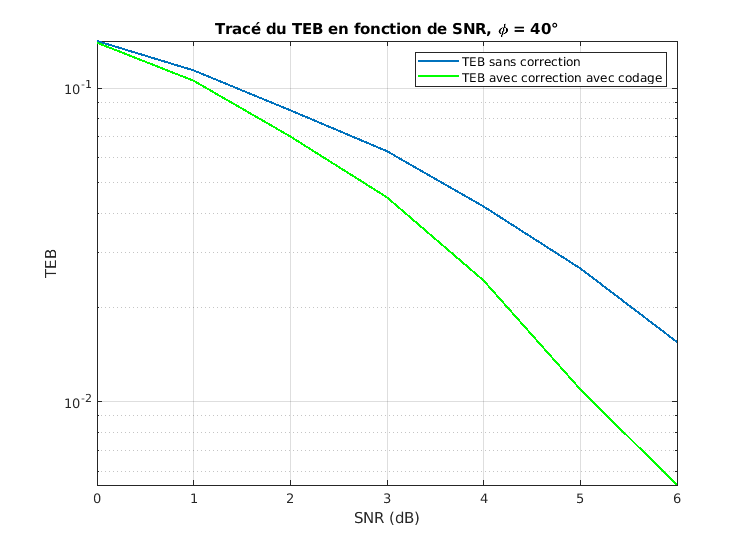
\includegraphics[height=7.8cm]{Screenshots/4_1_1.png}
    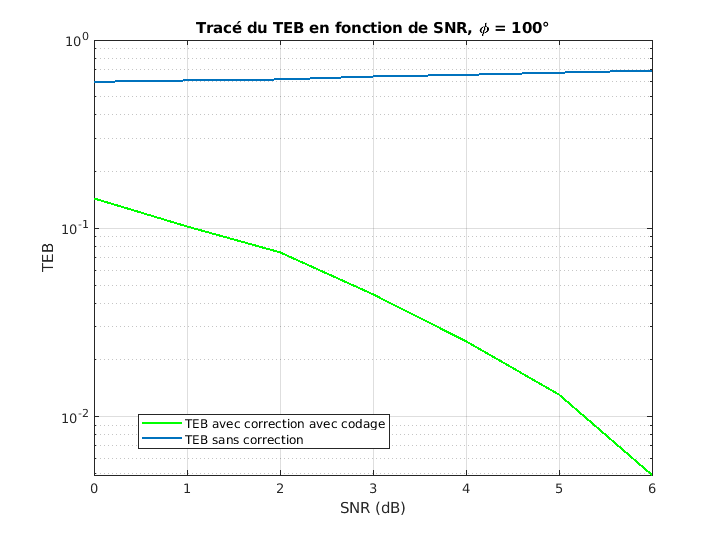
\includegraphics[height=7.8cm]{Screenshots/4_1_2.png}
    \caption{Comparaison des TEB simulés pour $\varphi = 40$° et $\varphi = 100$° avec codage par transition et correction de phase, et sans codage par transition ni correction de phase}
    \label{fig:un_label} 
\end{figure}

On remarque que pour $\phi = 40$° on obtient un meilleur TEB en utilisant la correction de phase et le codage source. Pour $\phi = 100$°, le TEB sans correction est trop elevé car les bits retrouvés sont inversés à cause du déphasage (>90°).

% Question 4.2.2

\begin{figure}[H]
    \centering
    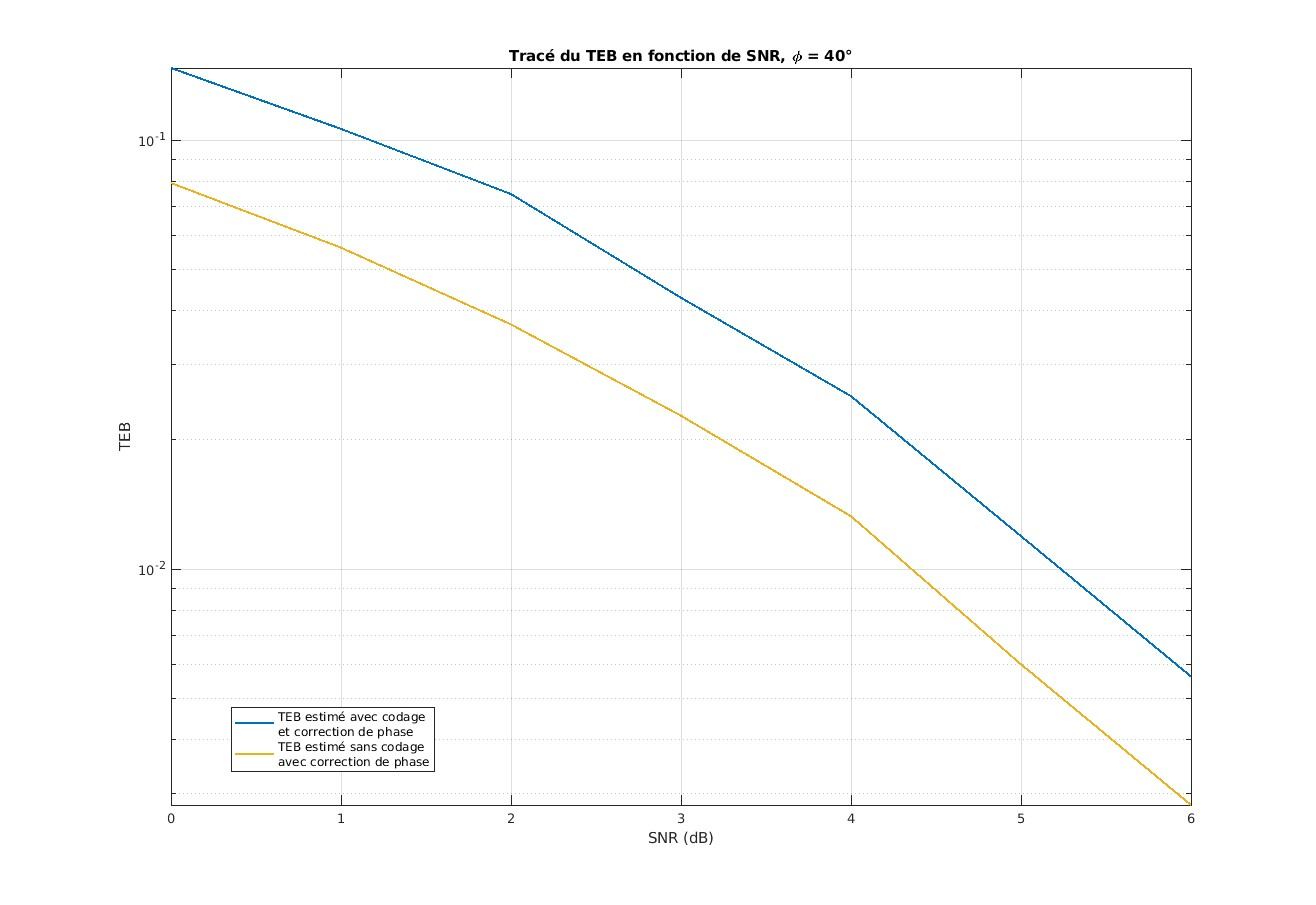
\includegraphics[height=7.8cm]{Screenshots/4_2_1.jpg}
    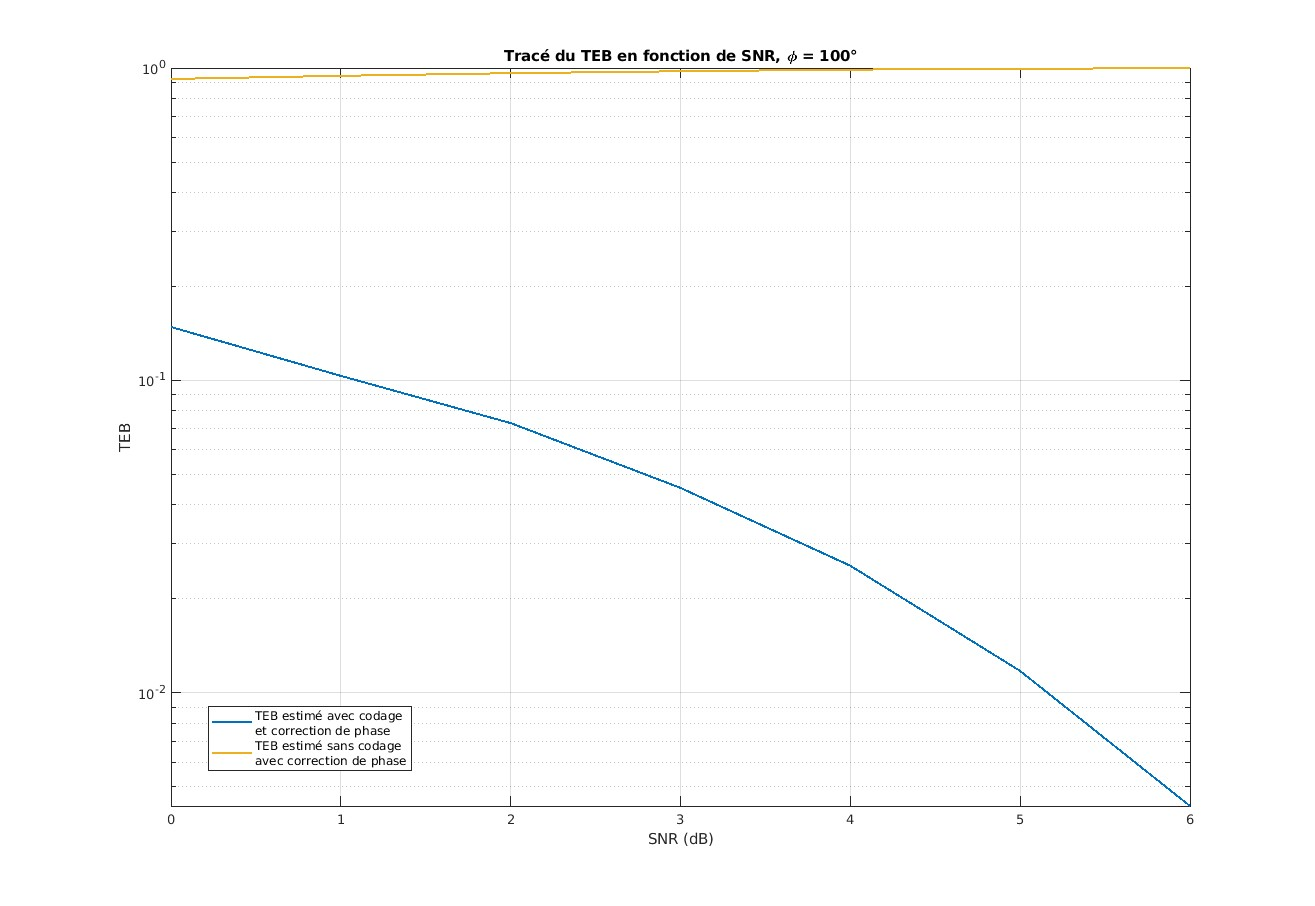
\includegraphics[height=7.8cm]{Screenshots/4_2_2.jpg}
    \caption{Comparaison des TEB simulés pour $\varphi = 40$° et $\varphi = 100$° avec correction de phase, avec et sans codage par transition}
    \label{fig:un_label} 
\end{figure}

On remarque que pour $\phi = 40$° on obtient un meilleur TEB en utilisant la correction de phase sans codage source. En effet, le TEB avec codage source est deux fois plus elevé que le TEB sans codage. Pour $\phi = 100$°, le TEB sans correction est trop elevé car les bits retrouvés sont inversés à cause du déphasage (>90°).

\part{Conclusion}
\fancyhead[C]{\nouppercase{\leftmark}}
\fancyhead[C]{Conclusion}
\renewcommand\thesection{\arabic{section}}

\section{Bilan}

Ce projet nous a permis de mettre en pratique les différentes notions acquises en cours. Nous avons eu l'opportunité de mettre en place une chaine de transmission avec erreur de phase, ce qui est le cas dans la réalité. Ensuite, nous avons vu comment estimer cette erreur de phase en utilisant l'estimateur de Viterbi et Viterbi ainsi que du codage source. Nous avons également pu observer l'impact de ces deux corrections sur la chaîne de transmission.

%\addtocontents{toc}{\setcounter{tocdepth}{0}}


\begin{thebibliography}{9}
\bibitem{misc}
Equipe pédagogique - Télécommunications (2023), \emph{Introduction aux Télécommunications - Introduction à la synchronisation - Impact d’une erreur de phase porteuse et méthode de récup ération}

\bibitem{misc}
Nathalie Thomas - Télécommunications (2023), \emph{Transmissions Bande de Base.}

\end{thebibliography}

\end{document}